\documentclass[12pt, letterpaper]{article}
\usepackage[utf8]{inputenc}
\usepackage{minted}
\usepackage{xcolor}
\usepackage[
  backend=biber,
  style=authortitle,
  autocite=footnote,
]{biblatex}
\addbibresource{references.bib}
\usepackage{setspace}
\onehalfspacing
\setminted{
    fontsize=\footnotesize,
    breaklines=true,
    linenos=true,
    framesep=2mm,
    baselinestretch=1
}
\usepackage{tikz}
\usetikzlibrary{positioning,arrows.meta}
\usepackage{hyperref}

\newcommand{\todo}[1]{\noindent\textcolor{red}{\textbf{\Large TODO: #1}}}
\newcommand{\note}[1]{\textcolor{red}{#1}}
\newcommand{\rough}[1]{\textcolor{blue}{Rough Notes: #1}}


\title{Implementation of Recursive Data Types in Modern Programming Languages}
\author{Josef Graf}
\date{\today}
\begin{document}
\maketitle

\newpage

\section{Introduction}
Recursive data types are a fundamental concept in computing, allowing for the representation of self-referential (recursive) types. By providing native support for them, programmers can easily represent complex structures such as trees without relying on fixed-size arrays or index-based representations, which are significantly more complicated. In this paper, we explore how various modern programming languages implement recursive data types, highlighting their syntax, semantics, and memory management techniques through the use of two examples.

Our first example is that of a tree where each node contains an integer value and optionally a left and right node of the same type.
\begin{minted}{go}
type Node {
  value: Int;
  left: Node | nil;
  right: Node | nil;
}
\end{minted}
We also define a recursive function \texttt{sum} that computes the sum of all values in the provided tree.
\begin{minted}{typescript}
function sum(root: Node): Int {
  acc := root.value;
  if (root.left != nil) {
    acc := acc + sum(root.left);
  }
  if (root.right != nil) {
    acc := acc + sum(root.right);
  }
  return acc;
}
\end{minted}
Finally, we illustrate how such trees are constructed, modified, and deconstructed through the following example.
\begin{minted}{go}
tree := Node(1, Node(2, nil, nil), Node(3, nil, nil));
total := sum(tree); // 6
tree.right := nil; // tree is now Node(1, Node(2, nil, nil), nil)
tree := tree.left; // Node(2, nil, nil)
\end{minted}

In our second example, we illustrate an abstract syntax tree (AST) for simple arithmetic expressions involving addition and multiplication.
\begin{minted}{haskell}
type Ast = Add(Ast, Ast) | Mul(Ast, Ast) | Num(String);
\end{minted}
We also define a recursive function \texttt{eval} that computes the integer result of the expression represented by the provided AST. To do so, we assume the existence of a function \texttt{parseInt} that takes a string as its sole parameter and returns the parsed integer value.
\begin{minted}{typescript}
function eval(expr: Ast): Int {
  switch expr {
    Add(left, right) => eval(left) + eval(right),
    Mul(left, right) => eval(left) * eval(right),
    Num(num) => parseInt(num),
  }
}
\end{minted}
Finally, we assume the existence an AST parsing function \texttt{parse} and use it to illustrate AST evaluation through the expression \texttt{2 + 3 * (4 + 5)}.
\begin{minted}{typescript}
expr := parse("2 + 3 * (4 + 5)") // Add(Num("2"), Mul(Num("3"), Add(Num("4"), Num("5"))))
result := eval(expr); // 29
\end{minted}

As a final note, all memory layout diagrams in this paper assume a 64-bit architecture with 8-byte pointers.

\section{Languages}
\subsection{Rust}
Rust is a statically typed, compiled language that relies on an ownership and borrowing system to provide memory safety without the need for a garbage collector.\autocite{rust-book} Rust has two core forms of custom data types relevant to this paper: structs and enums, defined with the \texttt{struct} and \texttt{enum} keywords, respectively. Struct types allow the definition of product types, and enums allow the definition of sum types; both can be used for recursive data types. To write our tree example in Rust, we would start with a struct \texttt{Node} and define our fields.\autocites[\href{https://doc.rust-lang.org/book/ch05-00-structs.html}{chap.~5}]{rust-book}[\href{https://doc.rust-lang.org/book/ch06-00-enums.html}{chap.~6}]{rust-book}[\href{https://doc.rust-lang.org/stable/reference/types.html}{\S~10.1}]{rust-reference}
\begin{minted}{rust}
struct Node {
    value: i32,
    left: Option<Box<Node>>,
    right: Option<Box<Node>>,
}
\end{minted}
The \texttt{Node} type takes 24 bytes, 8 for each of our left and right fields, 4 for our value field, and 4 bytes to ensure the struct's fields are aligned to an 8-byte boundary according to Rust's layout rules. Note that since Rust manages all field accesses itself and does not expose raw pointers as a safe API, the compiler may order the fields in any order when using the default representation.\autocite[\href{https://doc.rust-lang.org/stable/reference/type-layout.html}{\S~10.3}]{rust-reference}
\begin{figure}[H]
	\centering
	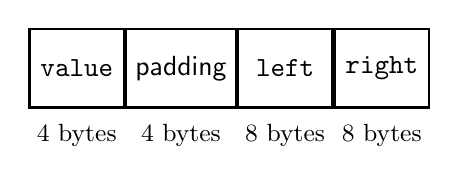
\begin{tikzpicture}[font=\sffamily, seg/.style={draw, thick, minimum height=1cm, minimum width=1.2cm, align=center}]
		\node[seg] (value) {\texttt{value}};
		\node[below=2pt of value, font=\small] {4 bytes};
		\node[seg, right=0cm of value] (padding) {padding};
		\node[below=2pt of padding, font=\small] {4 bytes};
		\node[seg, right=0cm of padding] (left) {\texttt{left}};
		\node[below=2pt of left, font=\small] {8 bytes};
		\node[seg, right=0cm of left] (right) {\texttt{right}};
		\node[below=2pt of right, font=\small] {8 bytes};
	\end{tikzpicture}
	\caption{Layout of \texttt{Node}}
\end{figure}

Since all types in Rust are stack allocated by default\autocite[\href{https://doc.rust-lang.org/rust-by-example/std/box.html}{\S~19.1}]{rust-example}, Rust requires that types, except for dynamically sized types, which we will not touch on here, have a known size at compile time.\autocite[\href{https://doc.rust-lang.org/book/ch20-03-advanced-types.html}{chap.~20~\S~3}]{rust-book} A byproduct of this rule is that recursive data types require some form of indirection, i.e., types cannot directly have fields of their same type; rather, they must be wrapped in another type with a known size.\autocite[\href{https://doc.rust-lang.org/stable/reference/types.html}{\S~10.1}]{rust-reference} When allocating on the heap, Rust provides the \texttt{Box<T>} type, which is a smart pointer to a heap-allocated instance of type \texttt{T}.\autocite[\href{https://doc.rust-lang.org/rust-by-example/std/box.html}{\S~19.1}]{rust-example} Thus, by using \texttt{Box<Node>} as the type of the left and right fields in \texttt{Node}, we are able to create recursive data types. However, if we used \texttt{Box<Node>}, then our tree would always be required to have both left and right nodes. To address this, we introduce the \texttt{Option<T>} type, a built-in enum that can be either \texttt{Some(T)} or \texttt{None}. By doing so, Rust programmers can pattern match using constructs such as \texttt{match} and \texttt{if let} to safely unpack an optional type.\autocite[\href{https://doc.rust-lang.org/book/ch06-00-enums.html}{chap.~6}]{rust-book} Conveniently, the Rust compiler also implements null-pointer optimization for \texttt{Option<Box<T>}, meaning that since \texttt{Box<T>} compiles down to a non-zero pointer, \texttt{Option<Box<T>} can be represented in the same space as a single pointer, using the null pointer to represent the \texttt{None} variant.\autocites{rust-boxed}{rust-option}
\begin{minted}{rust}
// the following are provided as simplified definitions of the Option and Box types included in Rust's standard library
enum Option<T> {
    Some(T),
    None,
}

struct Box<T> {
    ptr: *const T, // non-zero pointer to a heap allocated instance of type T
}
\end{minted}

Before we can implement our \texttt{sum} function, we first need a brief understanding of Rust's ownership and borrowing system, as well as deref coercion. This system enables the compiler to ensure memory safety by eliminating various classes of memory errors at compile time, without requiring a garbage collector or manual memory management. In Rust, each value has exactly one owner, and when that owner goes out of scope, the value is dropped, meaning Rust runs its destructor and deallocates any memory used by the value. Values can be borrowed through either mutable or immutable references; however, the compiler requires that each value have only a single mutable reference or any number of immutable references at any given time. Finally, references are also limited by the scope of the owner, meaning that a reference cannot outlive the value it is referencing.\autocite[\href{https://doc.rust-lang.org/book/ch04-00-understanding-ownership.html}{chap.~4}]{rust-book} Deref coercion is a key compiler feature that allows it to automatically convert between references to types that implement the \texttt{Deref} trait, allowing the programmer to use a \texttt{Box<T>} as if it were a reference \texttt{\&T}, or treat a \texttt{\&Option<T>} as a \texttt{Option<\&T>}.\autocite[\href{https://doc.rust-lang.org/book/ch15-02-deref.html}{chap.~15~\S~2}]{rust-book}

With this in mind, we now move to the definition of \texttt{sum}. The function takes a reference to a \texttt{Node} and, utilizing Rust's \texttt{if let} pattern matching and deref coercion, unpacks the optional left and right nodes to recursively sum the values of all nodes in the tree.
\begin{minted}{rust}
fn sum(node: &Node) -> i32 {
    let mut acc = node.value;
    if let Some(left) = &node.left {
        acc += sum(left);
    }
    if let Some(right) = &node.right {
        acc += sum(right);
    }
    acc
}
\end{minted}

In order to illustrate tree modification, we define our \texttt{tree} variable as mutable using the \texttt{mut} keyword. Then, we construct our left and right nodes, explicitly wrapping each in \texttt{Some} and a \texttt{Box::new} call to heap allocate them.
\begin{minted}{rust}
fn main() {
    let mut tree = Node {
        value: 1,
        left: Some(Box::new(Node {
            value: 2,
            left: None,
            right: None,
        })),
        right: Some(Box::new(Node {
            value: 3,
            left: None,
            right: None,
        })),
    };
\end{minted}
When calling \texttt{sum}, we pass a reference to our tree using the \texttt{\&} operator.
\begin{minted}{rust}
    let total = sum(&tree); // 6
\end{minted}
To remove the right node, we assign \texttt{None} to the \texttt{right} field, which causes the compiler to implicitly drop the previous right node (since it is moved out of \texttt{tree}, but not into a variable).\autocite[\S 15.2.2]{rust-example}
\begin{minted}{rust}
    tree.right = None; // tree is now Node { value: 1, left: Some(...), right: None }
\end{minted}
Finally, to deconstruct the tree and take ownership of the left node, we assign \texttt{tree.left} to a new variable \texttt{left}, causing a partial move, disallowing further access to \texttt{tree.left} for the remainder of the program and leaving us with an \texttt{Option<Box<Node>>} (moved from the heap to the stack) in \texttt{left}. To extract the inner \texttt{Node}, we use the \texttt{Option::unwrap} method, which will panic (crash the program) if we have \texttt{None}, but safely return \texttt{T} if we have \texttt{Some(T)}.\autocite{rust-option} Finally, to move ownership of the inner \texttt{Node} out of the \texttt{Box<Node>} and into \texttt{left}, we dereference the \texttt{Box<Node>} using the \texttt{*} operator.\autocite{rust-boxed}
\begin{minted}{rust}
    let left = tree.left;
    let unwrapped = left.unwrap();
    tree = *unwrapped; // tree is now Node { value: 2, left: None, right: None }
}
\end{minted}

Rust does not provide its own allocator; instead, it relies on the system allocator. For example, on Linux, this is often the \texttt{malloc} and \texttt{free} provided by glibc. glibc utilizes a series of arenas, which enable it to support multi-threading by creating new arenas as contention for existing arenas increases. Each arena then contains its own set of heaps, which are contiguous regions of memory obtained from the operating system using \texttt{mmap} or \texttt{sbrk}. Heaps are further subdivided into chunks of various sizes and sorted into bins based on their size. Each bin contains a linked list of free chunks within that arena, allowing multiple threads to request memory from different arenas without contention and reuse memory without performing memory compaction, albeit at the risk of fragmentation. When a chunk is free, it contains metadata that includes pointers to the next and previous chunks in the bin, allowing \texttt{malloc} to easily find free chunks and \texttt{free} to easily add chunks to the appropriate bin without requiring any memory beyond the chunk itself.\texttt{glibc}

Below is a diagram illustrating a simplified memory layout of our stack and heap after deconstructing our tree, but before final cleanup.
\begin{figure}[H]
	\centering
	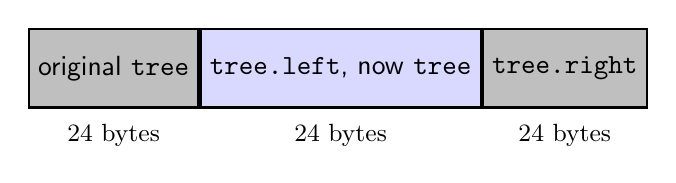
\begin{tikzpicture}[font=\sffamily, seg/.style={draw, thick, minimum height=1cm, minimum width=1.2cm, align=center}]
		\node[seg, fill=gray!50] (tree) {original \texttt{tree}};
		\node[below=2pt of tree, font=\small] {24 bytes};
		\node[seg, fill=blue!15, right=0cm of tree] (left) {\texttt{tree.left}, now \texttt{tree}};
		\node[below=2pt of left, font=\small] {24 bytes};
		\node[seg, fill=gray!50, right=0cm of left] (right) {\texttt{tree.right}};
		\node[below=2pt of right, font=\small] {24 bytes};
	\end{tikzpicture}
	\caption{Heap (gray = deallocated)}
\end{figure}
\begin{figure}[H]
	\centering
	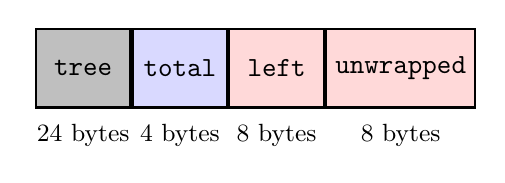
\begin{tikzpicture}[font=\sffamily, seg/.style={draw, thick, minimum height=1cm, minimum width=1.2cm, align=center}]
		\node[seg, fill=gray!50] (tree) {\texttt{tree}};
		\node[below=2pt of tree, font=\small] {24 bytes};
		\node[seg, fill=blue!15, right=0cm of tree] (total) {\texttt{total}};
		\node[below=2pt of total, font=\small] {4 bytes };
		\node[seg, fill=red!15, right=0cm of total] (left) {\texttt{left}};
		\node[below=2pt of left, font=\small] {8 bytes };
		\node[seg, fill=red!15, right=0cm of left] (unwrapped) {\texttt{unwrapped}};
		\node[below=2pt of unwrapped, font=\small] {8 bytes};
	\end{tikzpicture}
	\caption{Stack (gray = deallocated, red = moved)}
\end{figure}

This memory layout results in gaps on the heap. However, since Rust uses the system allocator and performs no automatic memory management itself, these gaps will be handled by the underlying allocator and potentially reused in the future according to its implementation.\autocite{rust-alloc}

Rust, however, is not limited to a single solution for type indirection; rather, it offers several options including typical heap allocation using (\texttt{Box<T>}, as we saw above), reference-counted types (\texttt{Rc<T>} or \texttt{Arc<T>}), and, of course, references (\texttt{\&T}). We have already covered \texttt{Box<T>}, so we now turn our attention to the remaining two.\autocite[\href{https://doc.rust-lang.org/book/ch15-00-smart-pointers.html}{chap.~15}]{rust-book}

Reference-counted types function more like garbage collection. The actual \texttt{Rc<T>} is only a pointer to the inner \texttt{T} and the count of active strong and weak references (stored as \texttt{RcInner<T>}). When a \texttt{Rc<T>} is cloned (a new instance is created referring to the same inner \texttt{T}), the inner strong reference count is incremented. When one is dropped (deallocated), the inner strong reference count is decremented through the \texttt{Drop} trait, analogous to a destructor. Weak references on the other hand, are created manually to handle potentially cyclic use cases. Since these types are part of the standard library (not compiler internals), when the reference count reaches zero, the inner memory is deallocated just like any other heap-allocated chunk of memory (i.e., handled by the system allocator). Rust has two such types, \texttt{Rc<T>} and \texttt{Arc<T}, the difference being that \texttt{Rc<T>} is restricted to a single thread and thus uses a plain location in memory to store its reference count, while \texttt{Arc<T>} can be sent safely between threads and uses an atomic internally for its reference count.\autocites[\href{https://doc.rust-lang.org/book/ch15-04-rc.html}{chap.~15~\S~4}]{rust-book}{rust-rc}{rust-arc}
\begin{figure}[H]
	\centering
	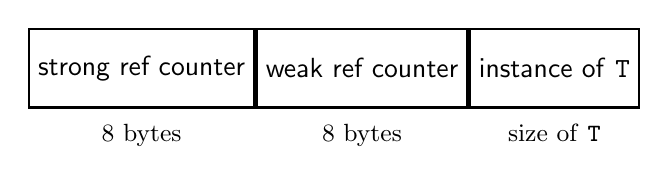
\begin{tikzpicture}[font=\sffamily, seg/.style={draw, thick, minimum height=1cm, minimum width=1.2cm, align=center}]
		\node[seg] (strong) {strong ref counter};
		\node[below=2pt of strong, font=\small] {8 bytes};
		\node[seg, right=0cm of strong] (weak) {weak ref counter};
		\node[below=2pt of weak, font=\small] {8 bytes};
		\node[seg, right=0cm of weak] (value) {instance of \texttt{T}};
		\node[below=2pt of value, font=\small] {size of \texttt{T}};
	\end{tikzpicture}
	\caption{Layout of \texttt{RcInner<T>}}
\end{figure}

Finally, references are a form of indirection that do not involve heap allocation or reference counting; instead, they are pointers to a value owned by another variable. However, to use references, we need to introduce the concept of lifetimes. In Rust, all references have a lifetime, i.e., the portion of code during which the reference is valid before the value it is referencing is dropped. The compiler can determine the lifetimes of many references on its own; however, defining types that contain references is not one of those cases. In order for a type to contain a reference, it must be constrained by that reference's lifetime.\autocites[\href{https://doc.rust-lang.org/book/ch04-02-references-and-borrowing.html}{chap.~4~\S~2}]{rust-book}[\href{https://doc.rust-lang.org/book/ch10-03-lifetime-syntax.html}{chap.~10~\S~3}]{rust-book} To demonstrate this, we use a variation of our AST example.

In this example, we define our AST using an enum following a similar pattern to our tree example, but with one key difference: the enum definition has a lifetime parameter \texttt{<'a>} and the \texttt{Num} variant contains a reference \texttt{\&'a str} rather than an owned \texttt{String}. These additions allow us to prevent unnecessary heap allocations and string copies, as we can tie the lifetime of our struct to that of the input string. Consequently, the Rust compiler ensures our AST cannot outlive the input string it references. This fact is exemplified by our \texttt{parse} function, which takes in a reference to a \texttt{str} (the primitive type Rust uses to refer to a length of string in memory) and returns an \texttt{Ast} tied to that same lifetime \texttt{'a}.\autocite[\href{https://doc.rust-lang.org/book/ch10-03-lifetime-syntax.html}{chap.~10~\S~3}]{rust-book}
\begin{minted}{rust}
enum Ast<'a> {
    Add(Box<Ast<'a>>, Box<Ast<'a>>),
    Mul(Box<Ast<'a>>, Box<Ast<'a>>),
    Num(&'a str),
}
\end{minted}
\begin{figure}[H]
	\centering
	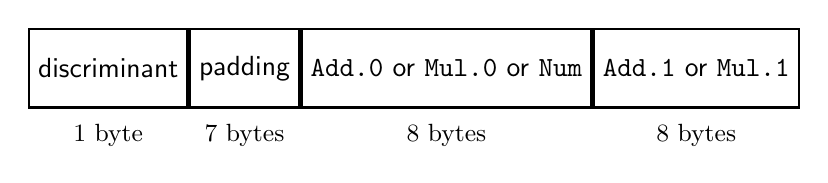
\begin{tikzpicture}[font=\sffamily, seg/.style={draw, thick, minimum height=1cm, minimum width=1.2cm, align=center}]
		\node[seg] (kind) {discriminant};
		\node[below=2pt of kind, font=\small] {1 byte};
		\node[seg, right=0cm of kind] (padding) {padding};
		\node[below=2pt of padding, font=\small] {7 bytes};
		\node[seg, right=0cm of padding] (left) {\texttt{Add.0} or \texttt{Mul.0} or \texttt{Num}};
		\node[below=2pt of left, font=\small] {8 bytes};
		\node[seg, right=0cm of left] (right) {\texttt{Add.1} or \texttt{Mul.1}};
		\node[below=2pt of right, font=\small] {8 bytes};
	\end{tikzpicture}
	\caption{Layout of \texttt{Ast<'a>}}
\end{figure}
\begin{minted}{rust}
fn eval(expr: &Ast) -> i32 {
    match expr {
        Ast::Add(left, right) => eval(left) + eval(right),
        Ast::Mul(left, right) => eval(left) * eval(right),
        Ast::Num(num) => num.parse::<i32>().unwrap(),
    }
}

fn parse<'a>(input: &'a str) -> Ast<'a> {
    unimplemented!()
}

fn main() {
    let expr = Ast::Add(
	Box::new(Ast::Num("2")),
	Box::new(Ast::Mul(
	    Box::new(Ast::Num("3")),
	    Box::new(Ast::Add(
		Box::new(Ast::Num("4")),
		Box::new(Ast::Num("5"))
	    ))
	))
    );
    let result = eval(&expr); // 29
}

fn will_error() {
    let expr;
    // we can use {...} to define a new scope
    {
        let expr_str = String::from("2 + 3 * (4 + 5)");
        expr = parse(&expr_str); // error: expr_str does not live long enough
    }
}
\end{minted}

When modifying an \texttt{Ast}, we can use similar patterns as before, but with the addition of pattern matching on enums. For example, to replace the left node of a \texttt{Add}, we would use the following:
\begin{minted}{rust}
let mut expr = Ast::Add(
    Box::new(Ast::Num("2")),
    Box::new(Ast::Num("3")),
);
if let Ast::Add(left, right) = &mut expr {
    *left = Box::new(Ast::Num("4"));
}
\end{minted}

In such a case, we use \texttt{if let} to match the correct variant, deref coercion, and then finally assign to the position in memory that \texttt{left} (a mutable reference) points to. Since our old value of \texttt{left} is no longer valid, the compiler will automatically drop it, and since Rust string literals are \texttt{\&'static str}, i.e., they are references to a sequence of bytes defined statically in the binary, we do not have to worry about lifetimes in this example.\autocite{rust-str}
\begin{figure}[H]
	\centering
	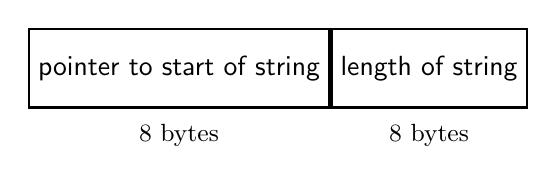
\begin{tikzpicture}[font=\sffamily, seg/.style={draw, thick, minimum height=1cm, minimum width=1.2cm, align=center}]
		\node[seg] (ptr) {pointer to start of string};
		\node[below=2pt of ptr, font=\small] {8 bytes};
		\node[seg, right=0cm of ptr] (len) {length of string};
		\node[below=2pt of len, font=\small] {8 bytes};
	\end{tikzpicture}
	\caption{Layout of \texttt{\&str}}
\end{figure}

In summary, \texttt{Box<T>} is the simplest solution, providing straightforward heap allocation with minimal overhead. It allows mutable and shared access, but is constrained by Rust's ownership and borrowing rules. It is best suited for situations where a single owner is required and heap allocation is an acceptable overhead (i.e., linked lists, trees, vectors, etc). \texttt{Rc<T>} and \texttt{Arc<T>} provide shared ownership through reference counting, allowing multiple parts of a program to have an owned reference to the same data. However, this comes with the overhead of managing the reference count. Since Rust requires sole ownership for mutable references, all data inside can only be accessed immutably unless wrapped in a type that provides interior mutability, such as a mutex. Reference-counted types are best suited for data that needs to be shared throughout the program or across threads (i.e., database connection pools), and the added overhead of managing the reference count is acceptable for the convenience compared to managing references and lifetimes manually. Finally, references (\texttt{\&T}) provide a zero-copy form of indirection that avoids heap allocations and reference counting entirely by pointing to an existing value. However, they are constrained by Rust's restrictions on borrowing and lifetimes, meaning they are best used as a temporary view into existing data when copying is too expensive (i.e., high-performance parsing or string manipulation).

\subsection{C}
C is a statically typed, compiled language that relies on manual memory management. C has three core forms of custom data types, structs, unions, and enums, defined with the \texttt{struct}, \texttt{union}, and \texttt{enum} keywords, respectively.

C requires that structs have a known size at compile time, but does not provide specialized smart pointer types for heap allocation or reference counting. Instead, C relies on the fixed size of raw pointers to achieve the required type indirection, requiring programmers to implement reference-counting themselves or through the use of external libraries.\autocite[\S~6.7.3.2]{c-standard} C also does not provide a built-in optional type and relies on the use of null pointers and manual null checks to represent optional values.\autocite[\S~6.3.2.3]{c-standard} To write our tree example in C using a struct \texttt{Node} and define our fields.\autocite[\S~6.~7]{c-standard}
\begin{minted}{c}
#include <stdlib.h>

struct Node {
  int value;
  struct Node *left;
  struct Node *right;
};
\end{minted}
\begin{figure}[H]
	\centering
	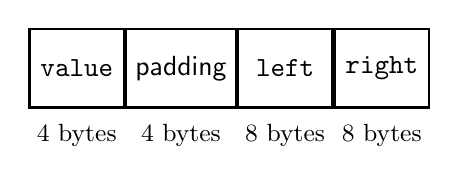
\begin{tikzpicture}[font=\sffamily, seg/.style={draw, thick, minimum height=1cm, minimum width=1.2cm, align=center}]
		\node[seg] (value) {\texttt{value}};
		\node[below=2pt of value, font=\small] {4 bytes};
		\node[seg, right=0cm of value] (padding) {padding};
		\node[below=2pt of padding, font=\small] {4 bytes};
		\node[seg, right=0cm of padding] (left) {\texttt{left}};
		\node[below=2pt of left, font=\small] {8 bytes};
		\node[seg, right=0cm of left] (right) {\texttt{right}};
		\node[below=2pt of right, font=\small] {8 bytes};
	\end{tikzpicture}
	\caption{Layout of \texttt{Node}}
\end{figure}

Our definition of \texttt{sum} takes a pointer to a \texttt{struct Node} and, utilizing basic null checks, recursively sums the values of all nodes in the provided tree.
\begin{minted}{c}
int sum(struct Node *node) {
  int acc = node->value;
  if (node->left != NULL) {
    acc += sum(node->left);
  }
  if (node->right != NULL) {
    acc += sum(node->right);
  }
  return acc;
}
\end{minted}

To construct our tree, we use the \texttt{malloc} function from C's standard library to allocate memory on the heap for each of our nodes. The C standard provides only broad guidance on the semantics of this allocation (or subsequent deallocation with \texttt{free}), so implementation design falls on the implementer, such as glibc.\autocite[\S~7.24.3]{c-standard} Once memory is allocated, we then use a compound literal to define our nodes and write them to the allocated memory.\autocite[\S~6.5.3.6]{c-standard}
\begin{minted}{c}
int main() {
  struct Node *tree = malloc(sizeof(struct Node));
  *tree = (struct Node){
    .value = 1,
    .left = malloc(sizeof(struct Node)),
    .right = malloc(sizeof(struct Node))
  };
  *tree->left = (struct Node){.value = 2, .left = NULL, .right = NULL};
  *tree->right = (struct Node){.value = 3, .left = NULL, .right = NULL};
\end{minted}

When calling \texttt{sum}, we pass our pointer to the root node and get out an integer result.
\begin{minted}{c}
  int total = sum(tree); // 6
\end{minted}

To remove our right node, we first free the memory used by the right node to prevent a memory leak, then we assign the \texttt{right} field to \texttt{NULL} to represent the absence of a node.\autocite[\S~7.24.3.3]{c-standard}
\begin{minted}{c}
  free(tree->right);
  tree->right = NULL; // tree is now Node { value: 1, left: ..., right: NULL }
\end{minted}

Finally, to deconstruct the tree and take ownership of the left node, we first assign \texttt{tree->left} to a new variable \texttt{tmp}, leaving us with a pointer to the left node in \texttt{left} and leaving our tree still intact. To fully deallocate the tree, we must manually call \texttt{free} on each of the nodes in the tree, which currently consists only of the root and its left child.
\begin{minted}{c}
  struct Node *tmp = tree->left;
  free(tree);
  tree = tmp; // tree is now Node { value: 2, left: NULL, right: NULL }
}
\end{minted}

In addition, since C uses null-terminated strings (a C string is a pointer to a sequence of bytes that ends with a null byte), C programmers cannot reference substrings without copying them into a new buffer. As such, we illustrate our AST example using owned strings rather than references.\autocite[\S~7.1.1]{c-standard} Since C does not have built-in tagged unions, we define our AST using a struct, a union, and an enum to represent the various node types.

First, we define \texttt{AstKind} to represent the type of each AST node; this is the tag for our tagged union.
\begin{minted}{c}
#include <stdlib.h>

enum AstKind { ADD, MUL, NUM };
\end{minted}
Next, we define our \texttt{AstData} union to represent the data for each of our node types.
\begin{minted}{c}
union AstData {
  struct {
    struct Ast *left;
    struct Ast *right;
  } add;
  struct {
    struct Ast *left;
    struct Ast *right;
  } mul;
  char *num;
};
\end{minted}
Finally, we define our \texttt{Ast} struct to contain both our tag and union.
\begin{minted}{c}
struct Ast {
  enum AstKind kind;
  union AstData data;
};
\end{minted}
\begin{figure}[H]
	\centering
	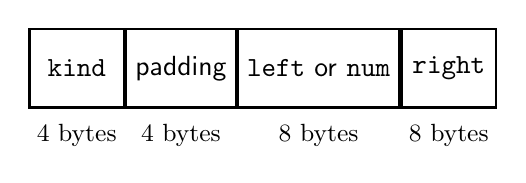
\begin{tikzpicture}[font=\sffamily, seg/.style={draw, thick, minimum height=1cm, minimum width=1.2cm, align=center}]
		\node[seg] (kind) {\texttt{kind}};
		\node[below=2pt of kind, font=\small] {4 bytes};
		\node[seg, right=0cm of kind] (padding) {padding};
		\node[below=2pt of padding, font=\small] {4 bytes};
		\node[seg, right=0cm of padding] (left) {\texttt{left} or \texttt{num}};
		\node[below=2pt of left, font=\small] {8 bytes};
		\node[seg, right=0cm of left] (right) {\texttt{right}};
		\node[below=2pt of right, font=\small] {8 bytes};
	\end{tikzpicture}
	\caption{Layout of \texttt{Ast}}
\end{figure}
To evaluate, we then use the \texttt{switch} statement to branch based on the tag and utilize C's built-in \texttt{atoi} function to parse integer values as needed.\autocite[\S~7.24.1.2]{c-standard}
\begin{minted}{c}
int eval(struct Ast *expr) {
  switch (expr->kind) {
  case ADD:
    return eval(expr->data.add.left) + eval(expr->data.add.right);
  case MUL:
    return eval(expr->data.mul.left) * eval(expr->data.mul.right);
  case NUM:
    return atoi(expr->data.num);
  default:
    return exit(1), 0; // unreachable)
  }
}

int main() {
  struct Ast *expr = malloc(sizeof(struct Ast));
  *expr = (struct Ast){
    .kind = ADD,
    .data.add = {
      .left = &(struct Ast){.kind = NUM, .data.num = "2"},
      .right = &(struct Ast){
        .kind = MUL,
        .data.mul = {
        .left = &(struct Ast){.kind = NUM, .data.num = "3"},
	  .right = &(struct Ast){
	    .kind = ADD,
	    .data.add = {
	      .left = &(struct Ast){.kind = NUM, .data.num = "4"},
	      .right = &(struct Ast){.kind = NUM, .data.num = "5"}
	    }
	  }
	}
      }
    }
  };
  int result = eval(expr); // 29
}
\end{minted}

If we wish to modify an \texttt{Ast}, we can use similar patterns as before. For example, to replace the left node of an \texttt{ADD}, we would use the following:
\begin{minted}{c}
// ensure we have an ADD node, otherwise we could be writing to an incorrect field
if (expr->kind == ADD) {
  free(expr->data.add.left); // free the old left node to prevent a memory leak
  expr->data.add.left = malloc(sizeof(struct Ast));
  *expr->data.add.left = (struct Ast){.kind = NUM, .data.num = "4"};
}
\end{minted}

\subsection{Python}
Python is a dynamically typed, garbage-collected, interpreted language. In CPython (the principal and reference implementation), it uses reference counting with optional detection of cyclically linked garbage through a garbage collector.\autocite{python-data-model} Python allows for recursive data types through classes, which can be defined using the \texttt{class} keyword.

For our first example, we use a class \texttt{Node} and define our two fields, a constructor (the \texttt{\_\_init\_\_} method), and use the \texttt{None} object to represent the absence of a node.\autocite{python-classes}
\begin{minted}{python}
class Node:
    def __init__(self, value, left = None, right = None):
        self.value = value
        self.left = left
        self.right = right
\end{minted}
Since Python is dynamically typed, all variables store the \texttt{id} (which is the memory address in CPython) of a reference-counted object on the heap. Thus, there is no need to define specific fields or provide any type information to Python since this is all handled at runtime. As a consequence of this, Python class instances, by default, use a hash map (\texttt{\_\_dict\_\_}) mapping field names to values (object IDs) rather than fixed slots in memory. While this provides complete flexibility, it comes with significant memory and performance overhead compared to storing fields directly.\autocites{python-data-model}{python-type-obj}{python-structures}
\begin{figure}[H]
	\centering
	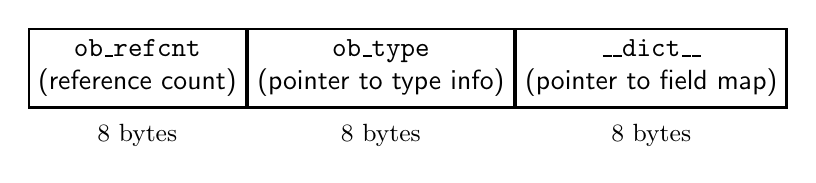
\begin{tikzpicture}[font=\sffamily, seg/.style={draw, thick, minimum height=1cm, minimum width=1.2cm, align=center}]
		\node[seg] (type) {\texttt{ob\_refcnt}\\(reference count)};
		\node[below=2pt of type, font=\small] {8 bytes};
		\node[seg, right=0cm of type] (refcnt) {\texttt{ob\_type}\\(pointer to type info)};
		\node[below=2pt of refcnt, font=\small] {8 bytes};
		\node[seg, right=0cm of refcnt] (dict) {\texttt{\_\_dict\_\_}\\(pointer to field map)};
		\node[below=2pt of dict, font=\small] {8 bytes};
	\end{tikzpicture}
	\caption{Simplified layout of a Python class instance}
\end{figure}
However, Python recognizes the performance implications of using a hash map for all field accesses and provides an alternative mechanism to define fixed fields using the \texttt{\_\_slots\_\_} attribute. By defining \texttt{\_\_slots\_\_}, Python will allocate space for each field inline in the object rather than using a hash map, improving both memory usage and performance, but at the cost of removing the ability to add new fields at runtime.\autocite[\S~3.3.2.4]{python-data-model}
\begin{minted}{python}
class NodeSlots:
    __slots__ = ['value', 'left', 'right']
    def __init__(self, value, left = None, right = None):
	self.value = value
	self.left = left
	self.right = right
\end{minted}
\begin{figure}[H]
	\centering
	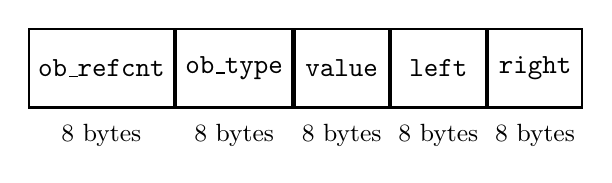
\begin{tikzpicture}[font=\sffamily, seg/.style={draw, thick, minimum height=1cm, minimum width=1.2cm, align=center}]
		\node[seg] (type) {\texttt{ob\_refcnt}};
		\node[below=2pt of type, font=\small] {8 bytes};
		\node[seg, right=0cm of type] (refcnt) {\texttt{ob\_type}};
		\node[below=2pt of refcnt, font=\small] {8 bytes};
		\node[seg, right=0cm of refcnt] (value) {\texttt{value}};
		\node[below=2pt of value, font=\small] {8 bytes};
		\node[seg, right=0cm of value] (left) {\texttt{left}};
		\node[below=2pt of left, font=\small] {8 bytes};
		\node[seg, right=0cm of left] (right) {\texttt{right}};
		\node[below=2pt of right, font=\small] {8 bytes};
	\end{tikzpicture}
	\caption{Simplified layout of a Python class instance with \texttt{\_\_slots\_\_}}
\end{figure}

Our definition of \texttt{sum} takes a \texttt{Node} and, utilizing the Python \texttt{is not} operator, checks for \texttt{None} to recursively sum the values of all nodes in the provided tree.
\begin{minted}{python}
def sum(node):
    acc = node.value
    if node.left is not None:
        acc += sum(node.left)
    if node.right is not None:
        acc += sum(node.right)
    return acc
\end{minted}

To construct our tree, we call the \texttt{Node} constructor, passing in the value and optionally the left and right nodes (which default to \texttt{None} if not provided). When allocating memory for objects, Python's memory manager first turns to the \texttt{pymalloc} allocator, a specialized allocator optimized for objects of size 512 bytes or less, which functions very similarly to glibc's \texttt{malloc} and \texttt{free}, utilizing arenas and pools (bins) to efficiently allocate blocks of memory while minimizing fragmentation. If the request is too large for \texttt{pymalloc}, Python falls back to the system allocator (i.e., \texttt{malloc} and \texttt{free} from glibc on Linux). Since CPython uses the system allocator and memory addresses as object IDs, no memory compaction is performed, as this would be incompatible with system allocator usage.\autocite{python-memory}
\begin{minted}{python}
tree = Node(1, Node(2), Node(3))
\end{minted}
When calling \texttt{sum}, we pass our tree and get out an integer result.
\begin{minted}{python}
total = sum(tree) # 6
\end{minted}
To remove our right node, we assign \texttt{None} to the \texttt{right} field of our tree, causing the reference count of the original right node to drop to zero, and thus causing it to be deallocated by Python's memory manager.
\begin{minted}{python}
tree.right = None # tree is now Node(1, Node(2), None)
\end{minted}
Finally, to deconstruct the tree into our left node, we assign the \texttt{left} field to our \texttt{tree} variable, causing the reference count of the original \texttt{tree} to drop to zero. However, the reference count of the left node stays at one since it is now being referred to by \texttt{tree}.
\begin{minted}{python}
tree = tree.left # tree is now Node(2)
\end{minted}

Similarly, we illustrate our AST example using classes. Since Python strings are immutable and do not allow storing zero-copy references to substrings, we use owned strings. Since Python does not have tagged unions, we will use Python classes to define our AST, using the built-in \texttt{isinstance} function to determine the type of each node.\autocite{python-classes}

First, we define each class similarly to our \texttt{Node} class, with each containing the appropriate fields and constructor.
\begin{minted}{python}
class Add:
    def __init__(self, left, right):
        self.left = left
        self.right = right
class Mul:
    def __init__(self, left, right):
        self.left = left
        self.right = right
class Num:
    def __init__(self, num):
        self.num = num
\end{minted}
When evaluating, we then use \texttt{isinstance} to determine the type of the node and recursively evaluate the appropriate fields, utilizing Python's built-in \texttt{int} function to parse integer values from strings stored in \texttt{Num}.\autocite{python-functions}
\begin{minted}{python}
def eval(expr):
    if isinstance(expr, Add):
        return eval(expr.left) + eval(expr.right)
    elif isinstance(expr, Mul):
        return eval(expr.left) * eval(expr.right)
    elif isinstance(expr, Num):
        return int(expr.num)

expr = Add(
    Num("2"),
    Mul(
	Num("3"),
	Add(
	    Num("4"),
	    Num("5")
	)
    )
)
result = eval(expr) # 29
\end{minted}

\subsection{Haskell}
Haskell is a statically typed, compiled, functional language that relies on garbage collection when using the Glasgow Haskell Compiler (GHC), the principal implementation of Haskell.\autocite[\S~5.7]{ghc} Rather than using structs, unions, enums, or classes, Haskell uses algebraic data types to define custom types, defined using the \texttt{data} keyword, that allow the definition of both product and sum types. To write our tree example in Haskell, we will use a data type \texttt{Node} and define our two fields.\autocite[\href{https://www.haskell.org/onlinereport/haskell2010/haskellch4.html}{chap.~4}]{haskell-report}

Since all values in Haskell are boxed by default (i.e., stored on the heap and accessed through a pointer), there is no need for any special pointer types to achieve indirection. Haskell also provides the \texttt{Maybe} type, a built-in type that can be either \texttt{Just a} or \texttt{Nothing}, to represent optional values.\autocites{haskell-heap}[\href{https://www.haskell.org/onlinereport/haskell2010/haskellch21.html}{chap.~21}]{haskell-report}
\begin{minted}{haskell}
data Node = Node {
  value :: Int,
  left :: Maybe Node,
  right :: Maybe Node
}
\end{minted}
\begin{figure}[H]
	\centering
	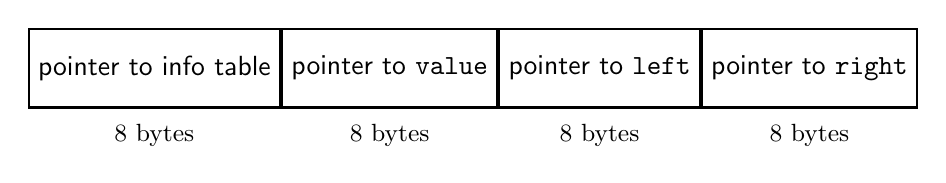
\begin{tikzpicture}[font=\sffamily, seg/.style={draw, thick, minimum height=1cm, minimum width=1.2cm, align=center}]
		\node[seg] (type) {pointer to info table};
		\node[below=2pt of type, font=\small] {8 bytes};
		\node[seg, right=0cm of type] (value) {pointer to \texttt{value}};
		\node[below=2pt of value, font=\small] {8 bytes};
		\node[seg, right=0cm of value] (left) {pointer to \texttt{left}};
		\node[below=2pt of left, font=\small] {8 bytes};
		\node[seg, right=0cm of left] (right) {pointer to \texttt{right}};
		\node[below=2pt of right, font=\small] {8 bytes};
	\end{tikzpicture}
	\caption{Layout of \texttt{Node}}
\end{figure}
\begin{figure}[H]
	\centering
	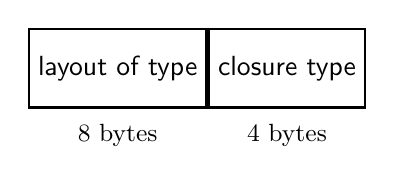
\begin{tikzpicture}[font=\sffamily, seg/.style={draw, thick, minimum height=1cm, minimum width=1.2cm, align=center}]
		\node[seg] (layout) {layout of type};
		\node[below=2pt of layout, font=\small] {8 bytes};
		\node[seg, right=0cm of layout] (type) {closure type};
		\node[below=2pt of type, font=\small] {4 bytes};
	\end{tikzpicture}
	\caption{Simplified layout of info table}
\end{figure}
By using the closure type and layout fields of the info table, Haskell can determine at runtime that the closure (object) is a \texttt{Node} and that it is composed of three fields, all pointers to other closures.\autocite{haskell-heap}

We define our \texttt{sum} function as \texttt{sumTree} to avoid overriding Haskell's built-in \texttt{sum} function. It then takes a \texttt{Node} and, utilizing Haskell's pattern matching, we unpack the optional left and right nodes to recursively sum the values of the entire tree.
\begin{minted}{haskell}
sumTree :: Node -> Int
sumTree (Node value Nothing Nothing) = value
sumTree (Node value (Just left) Nothing) = value + sumTree left
sumTree (Node value Nothing (Just right)) = value + sumTree right
sumTree (Node value (Just left) (Just right)) = value + sumTree left + sumTree right
\end{minted}

To construct our tree, we call the \texttt{Node} constructor, passing in the value and the left and right nodes as either \texttt{Just Node} or \texttt{Nothing}. When allocating memory for objects, GHC utilizes a generational garbage collector that divides the heap into multiple generations, thereby optimizing for the common case of short-lived objects. Objects are first allocated in a nursery before being promoted to older generations when the nursery fills up. The garbage collector periodically scans the heap to reclaim memory used by objects that are no longer reachable, copying live objects to new areas of memory to reduce fragmentation and enable the block allocator to perform compaction on empty blocks of memory.\autocite{ghc-gc}
\begin{minted}{haskell}
leftNode :: Node -> Maybe Node
leftNode (Node _ l _) = l
main :: IO ()
main = do
  let tree = Node 1 (Just (Node 2 Nothing Nothing)) (Just (Node 3 Nothing Nothing))
\end{minted}
When summing, we call our \texttt{sum} function with our tree.
\begin{minted}{haskell}
  let total = sumTree tree -- 6
\end{minted}
Since Haskell is a functional language, with immutable data types, to remove the right node, we create a new tree \texttt{tree2} using Haskell's record update syntax. Since Haskell does not allow variable reassignment, we must create a new variable rather than reassigning to \texttt{tree}.
\begin{minted}{haskell}
  let tree2 = tree { right = Nothing } -- tree2 is now Node 1 (Just (Node 2 Nothing Nothing)) Nothing
\end{minted}
Finally, to deconstruct the tree, we define a helper function \texttt{leftNode} that extracts the left node from a \texttt{Node} and then use it to assign the left node to a new variable \texttt{tree3}
\begin{minted}{haskell}
  let tree3 = leftNode tree -- tree3 is now Just (Node 2 Nothing Nothing)
  print total
\end{minted}

Since Haskell uses garbage collection, there is no need to free any memory manually, and the garbage collector automatically reclaims all memory used by the tree once it is no longer reachable, which will be after the \texttt{main} function ends.

Similarly, we illustrate our AST example using algebraic data types and pattern matching. Since Haskell strings are immutable, we use owned strings rather than zero-copy references to substrings.\autocite[\href{https://www.haskell.org/onlinereport/haskell2010/haskellch6.html}{chap.~6~\S1.2}]{haskell-report}

First, we define our AST using a single algebraic data type with three variants, each containing the required fields.
\begin{minted}{haskell}
data Ast = Add Ast Ast | Mul Ast Ast | Num String
\end{minted}
Each of the three variants are assigned a unique type in memory, allowing Haskell to determine which variant is being used through the closure type stored in the info table of the object.\autocite{haskell-heap}
\begin{figure}[H]
	\centering
	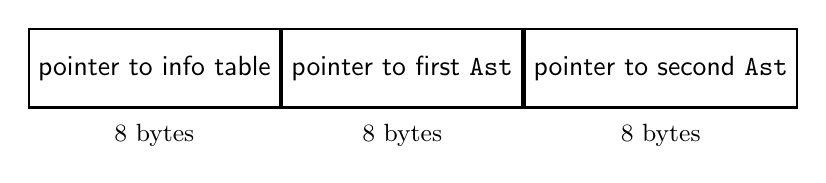
\begin{tikzpicture}[font=\sffamily, seg/.style={draw, thick, minimum height=1cm, minimum width=1.2cm, align=center}]
		\node[seg] (type) {pointer to info table};
		\node[below=2pt of type, font=\small] {8 bytes};
		\node[seg, right=0cm of type] (field1) {pointer to first \texttt{Ast}};
		\node[below=2pt of field1, font=\small] {8 bytes};
		\node[seg, right=0cm of field1] (field2) {pointer to second \texttt{Ast}};
		\node[below=2pt of field2, font=\small] {8 bytes};
	\end{tikzpicture}
	\caption{Layout of \texttt{Add}/\texttt{Mul}}
\end{figure}
\begin{figure}[H]
	\centering
	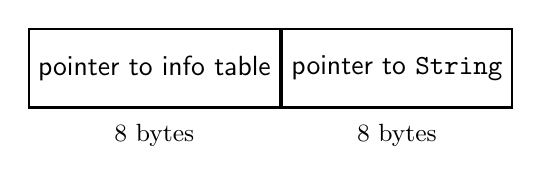
\begin{tikzpicture}[font=\sffamily, seg/.style={draw, thick, minimum height=1cm, minimum width=1.2cm, align=center}]
		\node[seg] (type) {pointer to info table};
		\node[below=2pt of type, font=\small] {8 bytes};
		\node[seg, right=0cm of type] (num) {pointer to \texttt{String}};
		\node[below=2pt of num, font=\small] {8 bytes};
	\end{tikzpicture}
	\caption{Layout of \texttt{Num}}
\end{figure}

To evaluate, we use Haskell's pattern matching syntax to branch over the variants and recursively evaluate the appropriate fields, utilizing Haskell's \texttt{read} function to parse integer values from the strings stored in \texttt{Num} variants.\autocite[\href{https://www.haskell.org/onlinereport/haskell2010/haskellch6.html}{chap.6~\S3.3}]{haskell-report}
\begin{minted}{haskell}
eval :: Ast -> Int
eval (Add left right) = eval left + eval right
eval (Mul left right) = eval left * eval right
eval (Num num) = read num :: Int
main :: IO ()
main = do
    let expr = Add (Num "2") (Mul (Num "3") (Add (Num "4") (Num "5")))
    let result = eval expr -- 29
    print result
\end{minted}

% \subsection{Zig}
% Zig is a statically typed, compiled language that relies on manual memory management. Similar to C, Zig has structs, unions, and enums defined with the \texttt{struct}, \texttt{union}, and \texttt{enum} keywords, respectively. To start, we write our tree example in Zig using a struct \texttt{Node} and define our fields.\autocite{zig-docs}
% \begin{minted}{zig}
% const Node = struct {
%     value: i32,
%     left: ?*Node,
%     right: ?*Node,
% };
% \end{minted}
% \begin{figure}[H]
% 	\centering
% 	\begin{tikzpicture}[font=\sffamily, seg/.style={draw, thick, minimum height=1cm, minimum width=1.2cm, align=center}]
% 		\node[seg] (value) {\texttt{value}};
% 		\node[below=2pt of value, font=\small] {4 bytes};
% 		\node[seg, right=0cm of value] (padding) {padding};
% 		\node[below=2pt of padding, font=\small] {4 bytes};
% 		\node[seg, right=0cm of padding] (left) {\texttt{left}};
% 		\node[below=2pt of left, font=\small] {8 bytes};
% 		\node[seg, right=0cm of left] (right) {\texttt{right}};
% 		\node[below=2pt of right, font=\small] {8 bytes};
% 	\end{tikzpicture}
% 	\caption{Layout of \texttt{Node}}
% \end{figure}
%
% Zig also requires that structs have a known size at compile time, and like C, it relies on the fixed size of raw pointers to achieve the required type indirection. Zig also has built-in optional types using the \texttt{?T} syntax. For optional pointer types (\texttt{?*T}), Zig uses null pointers to represent the absence of a value, similar to Rust and C.\autocite{zig-docs}
%
% Our \texttt{sum} function takes a pointer to a \texttt{Node} and, utilizing Zig's built-in optional type syntax, checks for \texttt{null} to recursively sum the values of all nodes in the provided tree.
% \begin{minted}{zig}
% fn sum(node: *const Node) i32 {
%     var acc = node.value;
%     if (node.left) |left| {
%         acc += sum(left);
%     }
%     if (node.right) |right| {
%         acc += sum(right);
%     }
%     return acc;
% }
% \end{minted}
%
% Finally, we illustrate tree construction, modification, and deconstruction through the following example. The \texttt{main} function runs at the start of a Zig program, and we use it here to construct our example tree, invoke our \texttt{sum} function, replace the right node, and finally deconstruct the tree.
%
% To construct our tree, we use the \texttt{std.heap} module from Zig's standard library to create a general-purpose allocator and allocate/destroy memory for each of our nodes. We then use a struct literal to define our nodes and write them to the allocated memory. We then use \texttt{defer} to ensure that the allocated memory is freed when the current scope ends.\autocite{zig-docs}
% \begin{minted}{zig}
% const std = @import("std");
%
% pub fn main() !void {
%     var gpa = std.heap.GeneralPurposeAllocator(.{}){};
%     const allocator = gpa.allocator();
%
%     var tree = try allocator.create(Node);
%     defer allocator.destroy(tree);
%     tree.value = 1;
%     tree.left = try allocator.create(Node);
%     tree.left.?.* = Node{ .value = 2, .left = null, .right = null };
%     defer if (tree.left) |left| allocator.destroy(left);
%     tree.right = try allocator.create(Node);
%     tree.right.?.* = Node{ .value = 3, .left = null, .right = null };
%     defer if (tree.right) |right| allocator.destroy(right);
% \end{minted}
%
% When calling \texttt{sum}, we pass our pointer to the root node and get out an integer result.
% \begin{minted}{zig}
%     const total = sum(tree); // 6
% \end{minted}
%
% Next, to remove our right node, we assign the \texttt{right} field to \texttt{null} to represent the absence of our right node. Since our initial deferred destruction of the right node only runs if \texttt{tree.right} is not null when \texttt{tree} goes out of scope, we must manually destroy \texttt{tree.right} before setting it to null in order to prevent a memory leak.
% \begin{minted}{zig}
%     if (tree.right) |right| allocator.destroy(right);
%     tree.right = null; // tree is now Node { value: 1, left: ..., right: null }
% \end{minted}
%
% Finally, to deconstruct the tree of the left node, we assign \texttt{tree.left} to a new variable \texttt{left}, leaving us with a pointer to the left node in \texttt{left} and leaving our tree still intact. Since we already deferred the destruction of the left node when we created it, it remains in memory until the end of the scope.
% \begin{minted}{zig}
%     const left = tree.left; // left is now Node { value: 2, left: null, right: null }
% }
% \end{minted}
%
% Similar to C, Zig does not provide built-in reference counting or other memory management schemes. However, unlike C, Zig does provide built-in tagged unions, allowing us to define our AST example more simply.
%
% First, we define our AST using a tagged union, with each variant containing the appropriate fields. By using the \texttt{[]const u8} type, we can refer to a slice of a string similar to Rust, allowing safe zero-copy string references. Then, when evaluating, we use Zig's \texttt{switch} expression to branch based on the tag and recursively evaluate the appropriate fields, utilizing Zig's built-in \texttt{std.fmt.parseInt} function to parse integer values from strings stored in \texttt{Num}.\autocite{zig-docs}\autocite{zig-parseint}
% \begin{minted}{zig}
% const std = @import("std");
% const Ast = union(enum) {
%     Add: struct { left: *Ast, right: *Ast },
%     Mul: struct { left: *Ast, right: *Ast },
%     Num: []const u8],
% };
%
% fn eval(expr: *const Ast) i32 {
%     return switch (expr.*) {
%         .Add => |add| eval(add.left) + eval(add.right),
%         .Mul => |mul| eval(mul.left) * eval(mul.right),
%         .Num => |num| std.fmt.parseInt(i32, num, 10),
%     };
% }
%
% fn parse(input: []const u8) *Ast {
%     return undefined;
% }
%
% pub fn main() !void {
%     const expr_str = "2 + 3 * (4 + 5)";
%     const expr = parse(expr_str);
%     const result = eval(&expr); // 29
% }
% \end{minted}


% \subsection{Go}
% Go is a statically typed, compiled language that relies on mark-sweep garbage collection. Go has structs and interfaces defined with the \texttt{struct} and \texttt{interface} keywords, respectively, but does not have built-in support for unions or enums. To write our tree example in Go, we will use a struct \texttt{Node} and define our two fields.\autocite{go-spec}
% \begin{minted}{go}
% package main
% type Node struct {
%     Value int
%     Left  *Node
%     Right *Node
% }
% \end{minted}
%
% Since Go is statically typed, it requires that structs have a known size at compile time, and like Rust and C, it relies on the fixed size of raw pointers to achieve the required type indirection. Go does not have a built-in optional type and relies on the use of the built-in \texttt{nil} value and manual nil checks to represent optional values.\autocite{go-spec}
%
% Now, we move to the definition of \texttt{sum}. The function takes a pointer to a \texttt{Node} and, utilizing basic nil checks, recursively sums the values of all nodes in the provided tree.
% \begin{minted}{go}
% func sum(node *Node) int {
%     acc := node.Value
%     if node.Left != nil {
%         acc += sum(node.Left)
%     }
%     if node.Right != nil {
%         acc += sum(node.Right)
%     }
%     return acc
% }
% \end{minted}
%
% Finally, we illustrate tree construction, modification, and deconstruction through the following example. The \texttt{main} function runs at the start of a Go program, and we use it here to construct our example tree, invoke our \texttt{sum} function, replace the right node, and finally deconstruct the tree.
%
% To construct our tree, we use Go's struct literal syntax to define our nodes and assign them to the required variables/fields; any missing fields are automatically initialized to the \texttt{nil} value for pointer types (which is the null pointer).\autocitethe request is too large for \texttt{pymalloc}, Python falls back to the system allocator ({go-spec}
% \begin{minted}{go}
% func main() {
%     tree := &Node{
%         Value: 1,
%         Left:  &Node{Value: 2},
%         Right: &Node{Value: 3},
%     }
% \end{minted}
%
% When calling \texttt{sum}, we pass our pointer to the root node and get out an integer result.
% \begin{minted}{go}
%     total := sum(tree) // 6
% \end{minted}
%
% Next, to remove our right node, we assign the \texttt{Right} field to \texttt{nil} to represent the absence of our right node, causing the garbage collector to reclaim the memory used by our right node on its next cycle since there are no other references to it.
% \begin{minted}{go}
%     tree.Right = nil // tree is now Node { Value: 1, Left: ..., Right: nil }
% \end{minted}
%
% Finally, to deconstruct the tree we assign \texttt{tree.Left} to a new variable \texttt{left}, leaving us with a pointer to the left node in \texttt{left} and leaves our tree still intact.
% \begin{minted}{go}
%     left := tree.Left // left is now Node { Value: 2, Left: nil, Right: nil }
% }
% \end{minted}
%
% Since Go uses garbage collection, there is no need to free any memory manually, and the garbage collector automatically reclaims all memory used by the tree once it goes out of scope.
%
% Similarly, we illustrate our AST example using structs, interfaces, and, since Go does not provide safe, zero-copy substrings, owned string values. Since Go does not have built-in tagged unions, we will use Go's type switch statement, similar to Python's \texttt{isinstance}, to determine the type of each node.\autocite{go-spec}
% \begin{minted}{go}
% package main
% import (
%     "strconv"
% )
% type Ast interface{}
% type Add struct {
%     Left Ast
%     Right Ast
% }
% type Mul struct {
%     Left Ast
%     Right Ast
% }
% type Num struct {
%     Value string
% }
% func eval(expr Ast) int {
%     switch e := expr.(type) {
%     case Add:
%         return eval(e.Left) + eval(e.Right)
%     case Mul:
%         return eval(e.Left) * eval(e.Right)
%     case Num:
%         n, _ := strconv.Atoi(e.Value)
%         return n
%     default:
%         panic("unreachable")
%     }
%   }
% func parse(input string) Ast {
%     // implementation omitted for simplicity
%     return nil
% }
% func main() {
%     // this may come from reading a file, user input, etc
%     expr_str := "2 + 3 * (4 + 5)"
%     expr := parse(expr_str)
%     result := eval(expr) // 29
% }
% \end{minted}
%
% First, we define an empty interface \texttt{Ast} to represent our AST nodes, then we define each variant as a struct containing the appropriate fields. Since our interface has no fields, all of our variant structs automatically implement the interface. Then, when evaluating, we use Go's type switch statement to branch based on the type of the node and recursively evaluate the appropriate fields, using Go's \texttt{strconv.Atoi} function to parse integer values from strings in \texttt{Num}.\autocite{go-spec}

\section{Conclusion}
Every language we have examined has offered a different set of features for memory management and recursive data types. C relies directly on raw pointers and manual memory management, providing maximum control but providing no protection against double-free, use-after-free, or memory leaks. On the opposite end of the spectrum, Haskell provides automatic garbage collection with built-in protection against reference cycles through its generational design. In the middle, we have languages like Rust, which guarantee memory safety through its ownership and borrowing system, preventing use-after-free and double-free vulnerabilities at compile time. Finally, Python provides automatic memory management through reference counting but does not have cycle detection by default.
\begin{table}[H]
	\centering
	\begin{tabular}{p{2cm}|p{3cm}|p{4cm}|p{3cm}}
		Language & Memory Management                          & Fragmentation                    & Allocator                               \\
		\hline
		Rust     & Ownership \& borrowing, reference counting & Yes, handled by system allocator & System (i.e., glibc)                    \\
		\hline
		C        & Manual                                     & Yes, handled by system allocator & System (i.e., glibc)                    \\
		\hline
		Python   & Reference counting                         & Yes, handled by system allocator & \texttt{pymalloc}, system (i.e., glibc) \\
		\hline
		Haskell  & Garbage collection                         & No, handled by garbage collector & Generational garbage collector          \\
	\end{tabular}
	\caption{Summary of memory management}
\end{table}
\begin{table}[H]
	\centering
	\begin{tabular}{p{3cm}|p{3cm}|p{3cm}|p{3cm}}
		Language         & Data Types             &
		Type Indirection & Optional Values                                                                                              \\
		\hline
		Rust             & Structs, enums         & \texttt{Box<T>}, \texttt{Rc<T>}, \texttt{Arc<T>}, \texttt{\&T} & \texttt{Option<T>} \\
		\hline
		C                & Structs, unions, enums & Raw pointers                                                   & Null Pointers      \\
		\hline
		Python           & Classes                & Object references                                              & \texttt{None}      \\
		\hline
		Haskell          & Algebraic data types   & Boxed values                                                   & \texttt{Maybe a}   \\
	\end{tabular}
	\caption{Summary of data types}
\end{table}

However, each memory management strategy comes with varying degrees of runtime overhead. Manual memory management, as in C, has no overhead beyond the cost of allocation and deallocation. Rust's ownership and borrowing system also has no runtime overhead since all code compiles down to manual memory management. However, reference counting through \texttt{Rc} and \texttt{Arc} incurs the overhead of incrementing and decrementing the reference count on clones and drops, with \texttt{Arc} also incurring the additional overhead of atomic operations to enable multi-threaded use. Python's reference counting also has the overhead of incrementing and decrementing the reference count, but unlike Rust, it has an optional garbage collector to detect cyclic references. Finally, Haskell's garbage collector has the most overhead since it must periodically stop the program to scan the heap for unreachable objects. However, Haskell's generational design allows it to optimize for the most common case of short-lived objects, enabling it to scan only certain generations rather than the entire heap on every run.
\begin{table}[H]
	\centering
	\begin{tabular}{p{2cm}|p{2cm}|p{4cm}|p{4cm}}
		Language                      & Runtime Overhead & Safety Guarantees                                                                                & Memory Footprint                                              \\
		\hline
		Rust (Ownership \& Borrowing) & None             & Prevents use-after-free and double-free at compile time, cycles cannot exist                     & Data                                                          \\
		\hline
		Rust (Rc/Arc)                 & Minor            & Prevents use-after-free and double-free at compile time, but no cycle detection                  & Pointer to ref count + data                                   \\
		\hline
		C                             & None             & No protection against use-after-free, double-free, or memory leaks, no protection against cycles & Data                                                          \\
		\hline
		Python                        & Minor            & Prevents use-after-free and double-free, but no cycle detection by default                       & Pointer to ref count + object + hash map + pointers to fields \\
		\hline
		Python (with GC)              & Significant      & Prevents use-after-free and double-free, prevents cycles                                         & Pointer to ref count + object + hash map + pointers to fields \\
		\hline
		Haskell                       & Significant      & Prevents use-after-free and double-free, prevents cycle                                          & Pointer to info table + pointers to fields                    \\
	\end{tabular}
	\caption{Summary of memory management and runtime overhead}
\end{table}

Overall, the choice of language and memory management strategy depends on the specific requirements of the application. For maximum control and performance, manual memory management in a language like C is the best choice; however, it comes with the potential for memory safety vulnerabilities. For safety and performance, but lacking the flexibility of raw pointers, Rust's ownership and borrowing system is ideal. For ease of use, the dynamic typing and automatic memory management of a language like Python are a great choice. However, they come with the overhead of an interpreter and reference counting, alongside the lack of type safety. Finally, for maximum safety and ease of use, a garbage-collected language like Haskell is an excellent choice. However, it comes with significant runtime overhead and lacks the control of manual memory management.

\newpage

\printbibliography

\end{document}
